\documentclass[a4paper, fontsize=12pt]{article}
\usepackage[english]{babel} % English language/hyphenation
\usepackage{amsmath,amsfonts,amsthm} % Math packages
\usepackage[utf8]{inputenc}
\usepackage{float}
\usepackage{lipsum} % Package to generate dummy text throughout this template
\usepackage{blindtext}
\usepackage{graphicx}
\usepackage{caption}
\usepackage{subcaption}
\usepackage[sc]{mathpazo} % Use the Palatino font
\usepackage[T1]{fontenc} % Use 8-bit encoding that has 256 glyphs
\linespread{1.05} % Line spacing - Palatino needs more space between lines
\usepackage{float} % Required for tables and figures in the multi-column environment - they need to be placed in specific locations with the [H] (e.g. \begin{table}[H])
\usepackage{hyperref} % For hyperlinks in the PDF
\usepackage{indentfirst}
\setlength{\parindent}{1.5em}
\usepackage{geometry}
\geometry{left=2cm,right=2cm,top=2.5cm,bottom=2.5cm}
\title{\vspace{-15mm}\fontsize{18pt}{10pt}\selectfont\textbf{HW 6}}
\author{Xinle Pang}
\date{\today}

\begin{document}
\maketitle % Insert title
\section{Question 1}
 $$V(w,p)=\max_{0\leq w'\leq w}p(w-w')-0.2(w-w')^1.5+\delta [V(w',p')|p],$$
 where $p'=p_{0}+\rho p +u', u \sim N(0,0.1^2)$.
 \begin{itemize}
 \item State variable: tree stock today $w$, price today $p$; choice variable:  tree stock tomorrow $w'$
 \item State space: $w \in [0,100]$
 
 
 \end{itemize}
\section{Question 3}
 \begin{figure}[H]
     \centering
     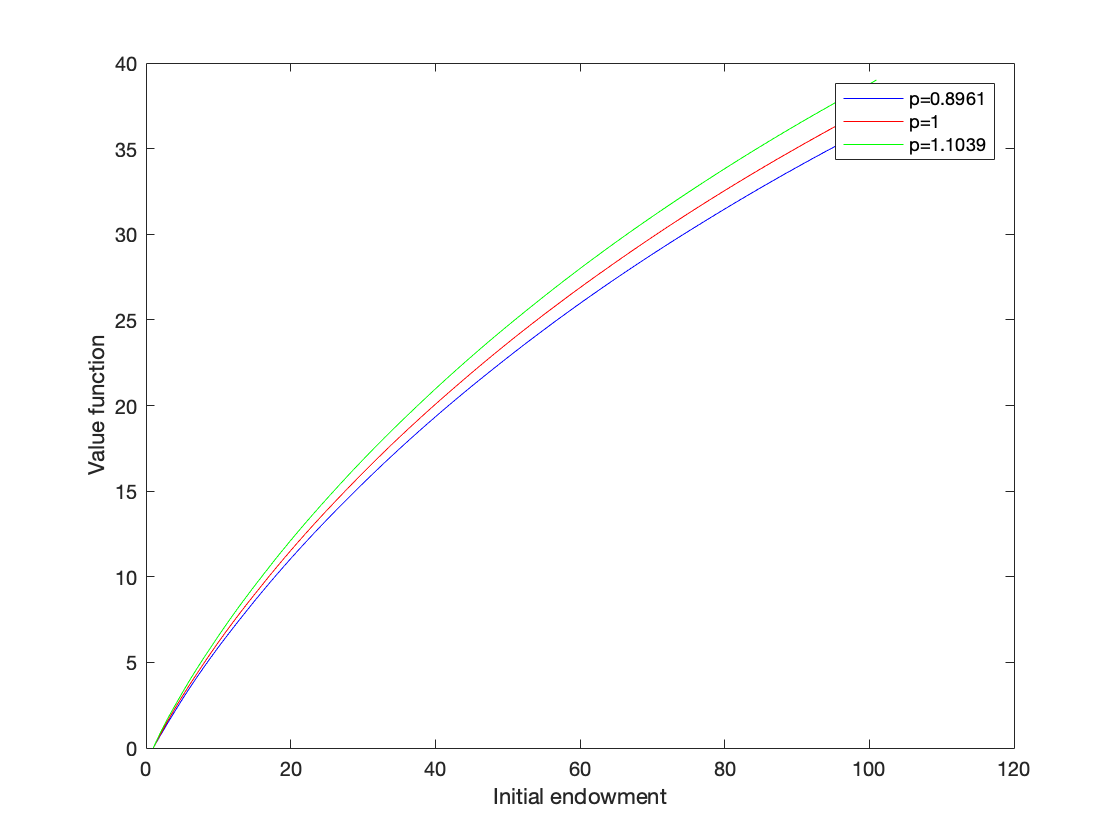
\includegraphics[width=9cm]{1.png}
 \end{figure}
\section{Question 4}
 \begin{figure}[H]
     \centering
     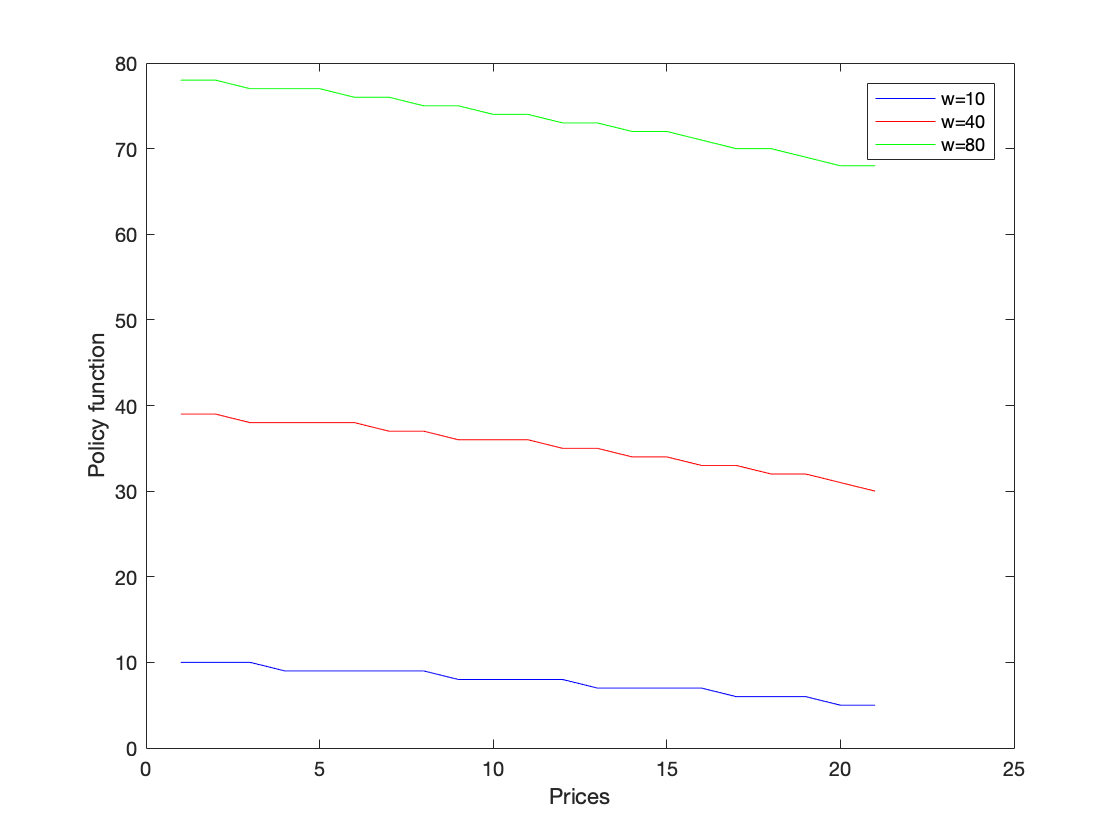
\includegraphics[width=9cm]{2.png}
 \end{figure}
 \section{Question 5}
 \begin{figure}[H]
     \centering
     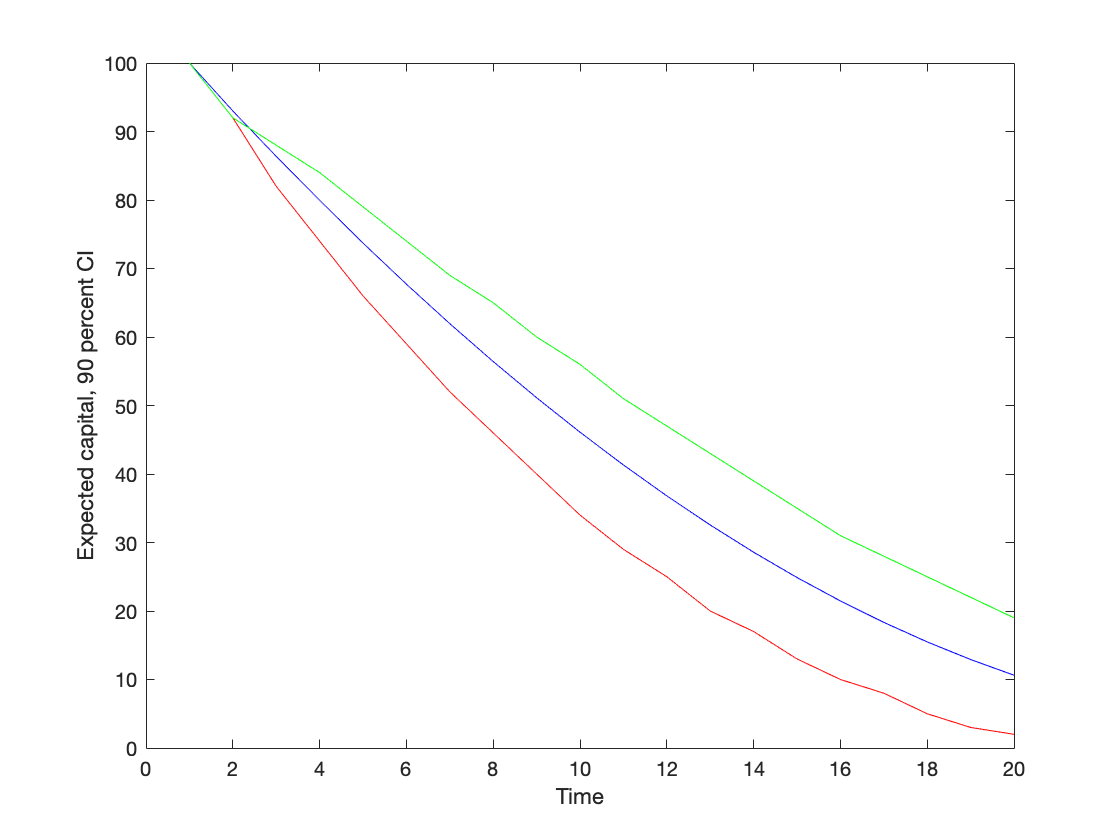
\includegraphics[width=9cm]{3.png}
 \end{figure}
 \section{Question 6}
 \begin{figure}[H]
     \centering
     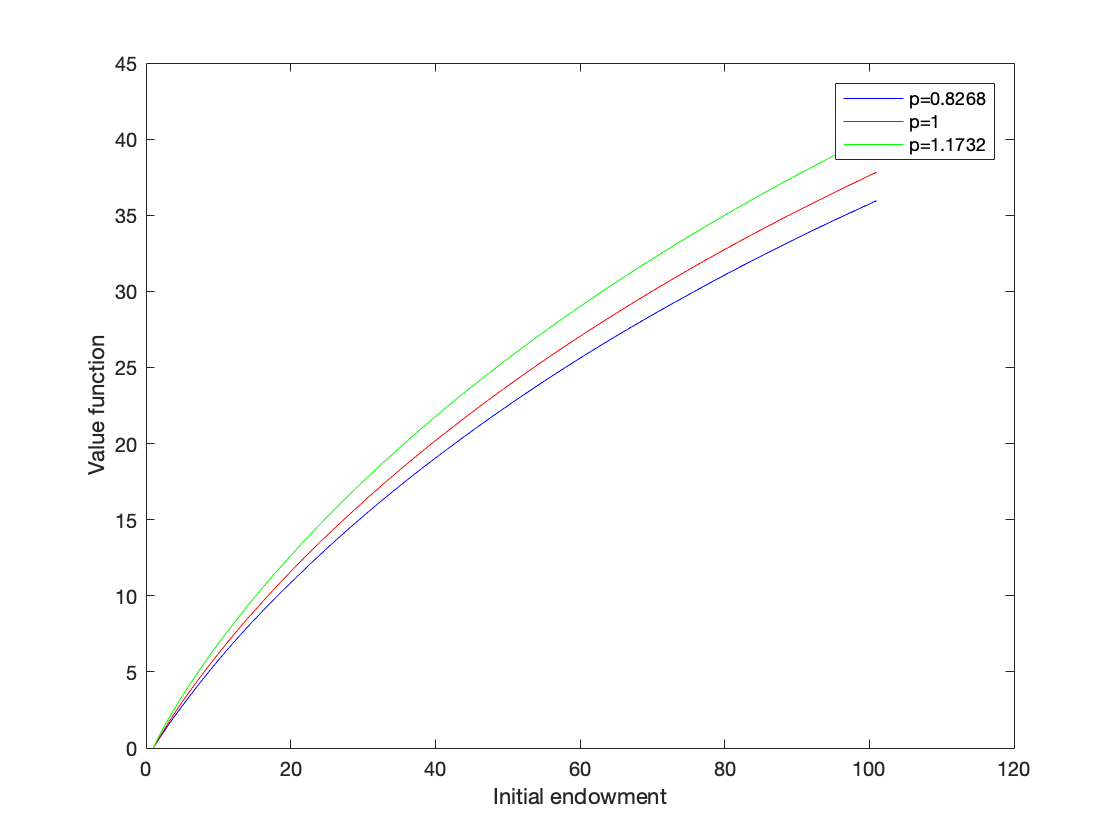
\includegraphics[width=9cm]{4.png}
 \end{figure}
  \begin{figure}[H]
     \centering
     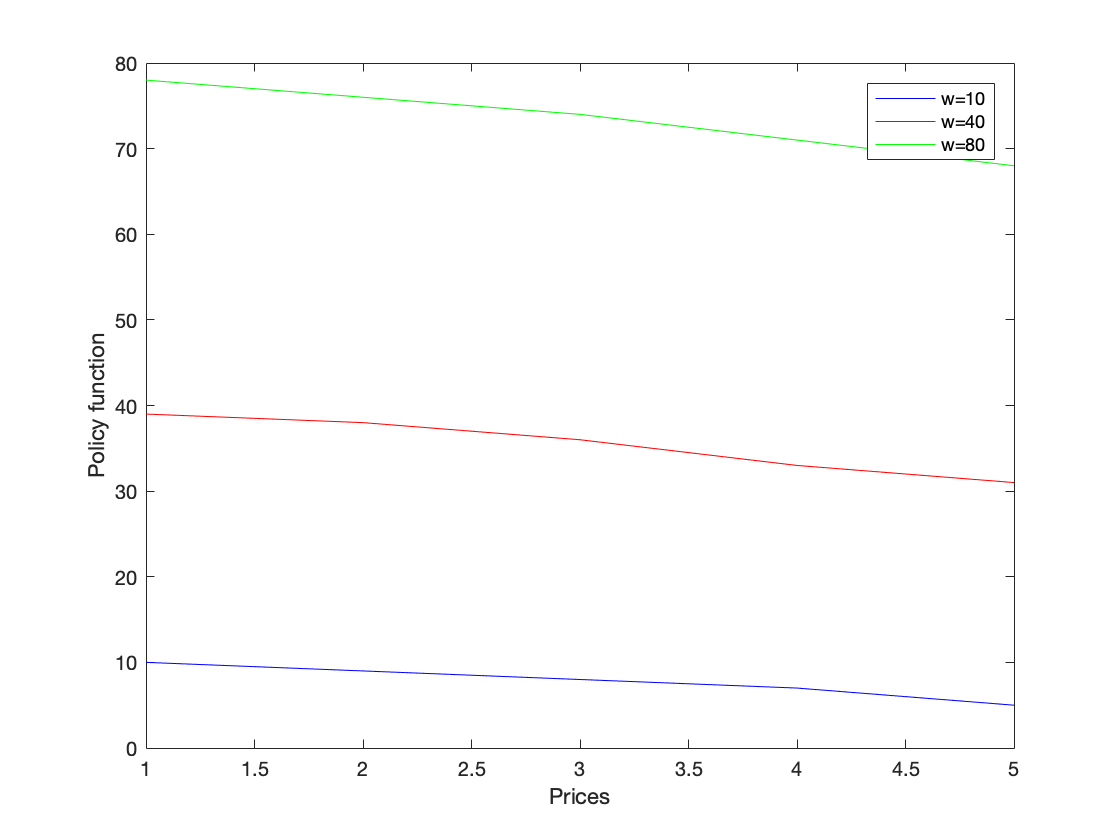
\includegraphics[width=9cm]{5.png}
 \end{figure}
\end{document}